% !TeX program = pdflatex
% !TeX encoding = utf8
% !TeX spellcheck = uk_UA
% !BIB program = bibtex8

\documentclass[18pt]{LectMechanics}
\usetikzlibrary{patterns, snakes}

\tikzset{
	body/.pic = {
			\fill[red!40, draw=red, opacity=0.5]  plot[smooth cycle, tension=.7] coordinates {
			(-2.5,0.5)
			(-0.5,2.5)
			(1.5,2)
			(2,0.5)
			(1,-1.5)
			(-1.5,-1.5)
		};
	}
}



\usetikzlibrary{arrows.meta}

\title[Physics 1]{\huge\bfseries Center of mass}
\date{}

\begin{document}
%=======================================================================================================
%\usebackgroundtemplate{
%
%\tikz\node[opacity=0.3]{\includegraphics[width=\paperwidth,height=\paperheight]{background}};%
%}
\begin{frame}
	\titlepage
\end{frame}
%=======================================================================================================
\usebackgroundtemplate{
}




%=======================================================================================================
\begin{frame}{Goals for Lecture}{}
	\begin{itemize}
		\item To uanderstand what is Center of mass
		\item To formulate thet theorem on the motion of the center of mass.
		\item Reference frame of the center of mass.
		\item Equation of motion of a body with a variable mass
	\end{itemize}
\end{frame}
%=======================================================================================================

%=======================================================================================================
\begin{frame}{What is CENETER OF MASS}{}
	\begin{columns}
		\begin{column}{0.5\linewidth}
			\only<1>{
				Any system of particles possesses one remarkable point $C$, the \emph{centre of inertia}, or the \emph{centre of mass}, displaying a number of interesting and significant properties. Its position relative to the origin $O$ of a given reference frame is described by the radius vector $\vec r_C$ defined by the following formula:
				\begin{equation*}
					\vec r_C = \frac{1}{M}\sum m_i \vec r_i
				\end{equation*}
				where $m_i$ and $\vec r_i$ are the mass and the radius vector of the $i$-ih particle, and $M$ is the mass of the whole system.}
			\only<2>{
				Differentiating last equation with respect to
				time, we get
				\begin{equation*}
					\vec V_C = \frac{1}{M}\sum m_i \vec v_i = \frac{1}{M}\sum \vec p_i
				\end{equation*}
				If the velocity of the centre of mass is equal to zero, the
				system is said to be at rest as a whole. This provides a
				natural generalization of the concept of a motionless particle.
				Accordingly, the velocity $\vec V_C$ acquires the meaning of the
				velocity of the system moving as a whole.}

		\end{column}
		\begin{column}{0.5\linewidth}
			\begin{overprint}
				\begin{tikzpicture}[scale=0.8, every node/.style={scale=0.8}]
					\draw[-latex, gray, thick] (0,0) -- +(1,0) node[right] {$y$};
					\draw[-latex, gray, thick] (0,0) -- +(0,1) node[left] {$z$};
					\draw[-latex, gray, thick] (0,0) -- +(-135:1) node[right] {$x$};
					\node[below] at (0,0) {$O$};

					\coordinate (B1) at (1,3);
					\coordinate (B2) at (4,5);
					\coordinate (B3) at (6,3);
					\coordinate (B4) at (4,1);

					\foreach \i in {1,...,4} {
							\draw[ball color=red!50] (B\i) circle (0.1);
							\draw[-latex, gray] (0,0) -- node[below] {$\vec r_{\i}$} (B\i);
							\draw[-latex, green!50!black] (B\i) -- +({180-30*\i}:1) node[above right] {$m_{\i}\vec v_{\i}$};
						}

					\draw[-latex, gray] let \p{B1}=(B1), \p{B2}=(B2), \p{B3}=(B3), \p{B4}=(B4) in
					(0,0) -- node[below] {$\vec r_{C}$} ({ (\x{B1} + \x{B2} + \x{B3} + \x{B4})/4 },{(\y{B1} + \y{B2} + \y{B3} + \y{B4})/4}) coordinate (C);

					\draw[ball color = gray] (C) circle (0.1) node[above] {$C$} node[below] {\small Center of Mass};
					\draw<2>[-latex] (C) -- +(135:1) node[above right] {$\vec V_C$};
				\end{tikzpicture}
			\end{overprint}
		\end{column}
	\end{columns}
\end{frame}
%=======================================================================================================

%=======================================================================================================
\begin{frame}{}{}
	From equation
	\begin{equation*}
		\vec V_C = \frac{1}{M}\sum m_i \vec v_i = \frac{1}{M}\sum \vec p_i
	\end{equation*}
	we get
	\begin{equation*}
		\vec P = M\vec V_C
	\end{equation*}
	i.e. the momentum of a system is equal to the product of the
	mass of the system by the velocity of its centre of mass.

\end{frame}
%=======================================================================================================

%=======================================================================================================
\begin{frame}{The equation of motion for the centre of mass}{}
	\only<1>{
		The concept of a centre of mass allows equation of moution of particle system:
		\begin{equation*}
			\frac{d\vec P}{dt} = \vec F^{ext}
		\end{equation*}
		to be rewritten in a more convenient form:
	}
	\begin{equation*}
		M\frac{d\vec V_C}{dt} = \vec F^{ext}
	\end{equation*}
	\only<1>{
		This is the equation of motion for the centre of inertia
		of a system. According to this equation, during the motion of any
		system of particles its centre of inertia moves as if all the mass
		of the system were concentrated at that point, and all external
		forces acting on the system were applied to it. In this case
		the acceleration of the centre of inertia is quite independent
		of the points to which the external forces are applied.
	}
	\only<2>{%
		\begin{columns}
			\begin{column}{0.5\linewidth}
				Next, it follows from this equation for the closed system $\vec F^{ext} = 0$, then
				$M\frac{d\vec V_C}{dt} = 0$, and therefore:

				\begin{equation*}
					\vec V_C = \mathrm{const}
				\end{equation*}

				Thus, if the centre of inertia of a system moves \emph{uniformly} and \emph{rectilinearly}, the momentum of the system remains constant in the process of motion. Obviously, the reverse statement is also true.
			\end{column}
			\begin{column}{0.5\linewidth}
				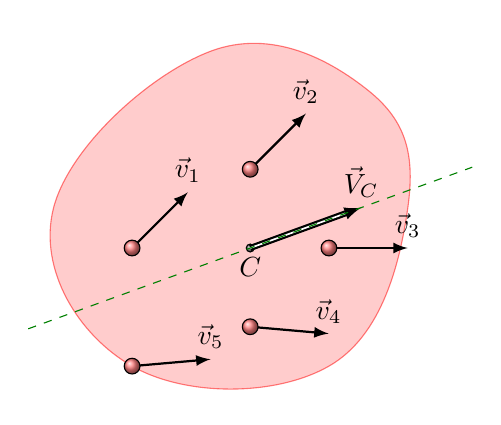
\begin{tikzpicture}
					\coordinate (O) at (0,0);
					% ====== Bodyes ========
					\coordinate (B1) at (2,2.5);
					\coordinate (B2) at (3.5,3.5);
					\coordinate (B3) at (4.5,2.5);
					\coordinate (B4) at (3.5,1.5);
					\coordinate (B5) at (2,1);
					\coordinate (C) at (3.5,2.5);
					\pgfmathsetmacro{\ang}{20}
					% ====== System ========
					\pic at (C) {body};
					\draw[-latex, thick] (B1) -- +(45:1) node[above] {$\vec v_1$};
					\draw[-latex, thick] (B2) -- +(45:1) node[above] {$\vec v_2$};
					\draw[-latex, thick] (B3) -- +(0:1) node[above] {$\vec v_3$};
					\draw[-latex, thick] (B4) -- +(-5:1) node[above] {$\vec v_4$};
					\draw[-latex, thick] (B5) -- +(5:1) node[above] {$\vec v_5$};

					\foreach \i in {1,...,5} {\draw[ball color=red!50] (B\i) circle (0.1);}
					\draw[ball color=gray] (C) circle (0.05) node[below] {$C$};
					\draw[-latex, thick, double] (C) -- +(\ang:1.5) node[above] {$\vec V_C$};
					\draw[green!50!black, dashed] ([shift={({180+\ang}:3)}]C) -- (C) -- ([shift={(\ang:3)}]C);
				\end{tikzpicture}
			\end{column}
		\end{columns}
	}
\end{frame}
%=======================================================================================================

%=======================================================================================================
\begin{frame}{Reference frame of the center of mass}{}
	Reference frame of the center of mass is the  \emph{reference frame in which the centre of inertia is at rest}. Using this frame we can significantly simplify both the analysis of phenomena and the calculations.
	\begin{columns}
		\begin{column}{0.5\linewidth}
			The reference frame rigidly fixed to the centre of mass of a given system of particles and translating with respect to inertial frames is referred to as the frame of the centre of mass. The distinctive feature of this frame is that the total momentum of the system of particles is equal to zero:
			\begin{equation*}
				\vec P_C = 0
			\end{equation*}
		\end{column}
		\begin{column}{0.5\linewidth}
			\begin{center}
				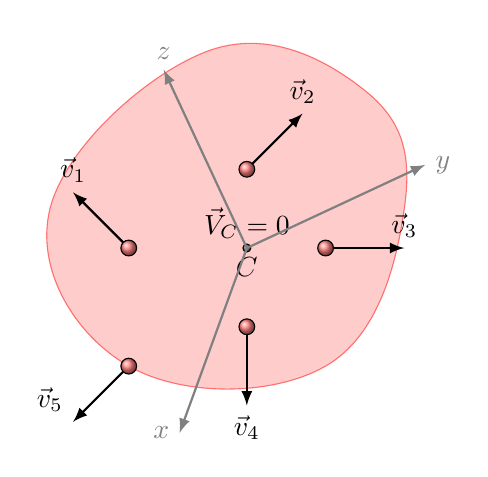
\begin{tikzpicture}
					\coordinate (O) at (0,0);
					% ====== Bodyes ========
					\coordinate (B1) at (2,2.5);
					\coordinate (B2) at (3.5,3.5);
					\coordinate (B3) at (4.5,2.5);
					\coordinate (B4) at (3.5,1.5);
					\coordinate (B5) at (2,1);
					\coordinate (C) at (3.5,2.5);
					\pgfmathsetmacro{\ang}{20}
					% ====== System ========
					\pic at (C) {body};
					\draw[-latex, thick] (B1) -- +(135:1) node[above] {$\vec v_1$};
					\draw[-latex, thick] (B2) -- +(45:1) node[above] {$\vec v_2$};
					\draw[-latex, thick] (B3) -- +(0:1) node[above] {$\vec v_3$};
					\draw[-latex, thick] (B4) -- +(-90:1) node[below] {$\vec v_4$};
					\draw[-latex, thick] (B5) -- +(225:1) node[above left] {$\vec v_5$};

					\foreach \i in {1,...,5} {\draw[ball color=red!50] (B\i) circle (0.1);}
					\draw[ball color=gray] (C) circle (0.05) node[below] {$C$};
					\node[above] at (C) {$\vec V_C = 0$} ;
					\begin{scope}[rotate = 25]
						\draw[thick, gray, -latex] (C) -- +(0,2.5) node[above, ] {$z$};
						\draw[thick, gray, -latex] (C) -- +(2.5,0) node[right] {$y$};
						\draw[thick, gray, -latex] (C) -- +(225:2.5) node[left] {$x$};
					\end{scope}

				\end{tikzpicture}
			\end{center}
		\end{column}
	\end{columns}
\end{frame}
%=======================================================================================================

%=======================================================================================================
\begin{frame}{A system of two particles}{Coordinates of the Center of mass}
	The coordinates of the centre of mass are:
	\begin{equation*}
		x_C = \frac{m_1 x_1 + m_2 x_2}{m_1 + m_2}, \quad y_C = \frac{m_1 y_1 + m_2 y_2}{m_1 + m_2}, \quad z_C = \frac{m_1 z_1 + m_2 z_2}{m_1 + m_2}
	\end{equation*}
	\begin{center}
		\begin{tikzpicture}
			\pgfmathsetmacro{\l}{6}
			\coordinate (B1) at (0,0);
			\coordinate (B2) at (\l,0);

			\draw[ball color=red!50] (B1) circle (0.5);
			\draw[ball color=red!50] (B2) circle (1.0);

			\draw[-latex, thick] (0,0) -- +(\l+2,0) node[right] {$x$};
			\node[mark size=5pt] at (B1) {\pgfuseplotmark{|}};
			\node[below=1cm] at (B1) {$x_1 = 0$ m};
			\node[above=1cm] at (B1) {$m_1 = 1$ kg};
			\node[mark size=5pt] at (B2) {\pgfuseplotmark{|}};
			\node[below=1cm] at (B2) {$x_2 = \l$ m};
			\node[above=1cm] at (B2) {$m_2 = 2$ kg};


			\draw let \p{B1}=(B1), \p{B2}=(B2) in ({2*\x{B2}/3}, 0) circle (0.1) node[mark size=0.1cm] {\pgfuseplotmark{|}} node[below=0.5cm] {$x_C = \pgfmathparse{2*\x{B2}/3*0.03514}\pgfmathprintnumber[precision=1]{\pgfmathresult}$ m};
		\end{tikzpicture}
	\end{center}
\end{frame}
%=======================================================================================================

\begin{frame}{A system of two particles}{Velocity of the Center of mass}
	The coordinates of the centre of mass are:
	\begin{equation*}
		V_{x_C} = \frac{m_1 v_{x_1} + m_2  v_{x_2}}{m_1 + m_2}, \quad V_{y_C} = \frac{m_1  v_{y_1} + m_2  v_{y_2}}{m_1 + m_2}, \quad V_{z_C} = \frac{m_1 v_{z_1} + m_2  v_{z_2}}{m_1 + m_2}
	\end{equation*}
	\begin{center}
		\begin{tikzpicture}
			\pgfmathsetmacro{\l}{6}
			\coordinate (B1) at (0,0);
			\coordinate (B2) at (\l,0);

			\draw[ball color=red!50] (B1) circle (0.5);
			\draw[ball color=red!50] (B2) circle (1.0);

			\draw[-latex, thick] (0,0) -- +(\l+2,0) node[right] {$x$};
			\node[mark size=1pt] at (B1) {\pgfuseplotmark{*}};
			\node[above=1cm] at (B1) {$m_1 = 1$ kg};
			\node[mark size=1pt] at (B2) {\pgfuseplotmark{*}};
			\node[above=1cm] at (B2) {$m_2 = 2$ kg};

			\draw[-latex, red, thick] (B1) -- +(-2,0) node[below=1cm] {$v_{x_1} = -2$~m/s};
			\draw[-latex, red, thick] (B2) -- +(-1,0) node[below=1cm] {$v_{x_2} = -1$~m/s};


			\draw let \p{B1}=(B1), \p{B2}=(B2) in ({2*\x{B2}/3}, 0) coordinate (C) circle (0.1) node[mark size=0.1cm] {\pgfuseplotmark{|}};
			\pgfmathsetmacro{\V}{(-1*2-2*1)/3}
			\draw[-latex, blue, double] (C) -- +(\V,0) node[below=0.5cm] {$\vec V_C = \pgfmathprintnumber[precision=2]{\V}$~m/s};
		\end{tikzpicture}
	\end{center}
\end{frame}
%=======================================================================================================

%=======================================================================================================
\begin{frame}{A system of two particles}{Momentum of the particles in the System of Center of Mass}

	\only<1>{
		Velocity of first particle relative to CM $\vec{\tilde{v}}_1 = \vec v_1 - \vec V_C = \frac{m_2(\vec v_1 - \vec v_2)}{m_1 + m_2}$.

		Velocity of second particle relative to CM $\vec{\tilde{v}}_2 = \vec v_2 - \vec V_C = \frac{m_1(\vec v_1 - \vec v_2)}{m_1 + m_2}$.

		\hrulefill

		Momentum of first particle relative to CM $\vec{\tilde{p}}_1 = m\vec{\tilde{v}}_1 =  \frac{m_1m_2}{m_1 + m_2}(\vec v_1 - \vec v_2)$.

		Momentum of second particle relative to CM $\vec{\tilde{p}}_2 = -m\vec{\tilde{v}}_2 =  \frac{m_1m_2}{m_1 + m_2}(\vec v_1 - \vec v_2)$.

		\hrulefill

		In reference frame of the CM:
		\begin{equation*}
			\vec{\tilde{p}}_1 = -\vec{\tilde{p}}_2
		\end{equation*}

		Or we can rewrite $\vec{\tilde{p}}_1$ or $\vec{\tilde{p}}_2$ in terms of relative velocity \emph{$\vec v_\mathrm{rel} = \vec v_1 - \vec v_2$} and reduced mass of the system 	\emph{$\mu = \frac{m_1m_2}{m_1 + m_2} $}:

		\begin{equation*}
			\vec{\tilde{p}}_1 = -\vec{\tilde{p}}_2 = \mu \vec v_\mathrm{rel}
		\end{equation*}
	}
	\only<2>{
		\begin{columns}
			\begin{column}{0.5\linewidth}
				Magnitude of momentum are equal
				\begin{equation*}
					\tilde{p}_1 = \tilde{p}_2 = \mu v_\mathrm{rel}
				\end{equation*}

				but directions are oposite:

				\begin{equation*}
					\vec{\tilde{p}}_2 \uparrow \downarrow \vec{\tilde{p}}_1
				\end{equation*}
			\end{column}
			\begin{column}{0.5\linewidth}
				\begin{center}
					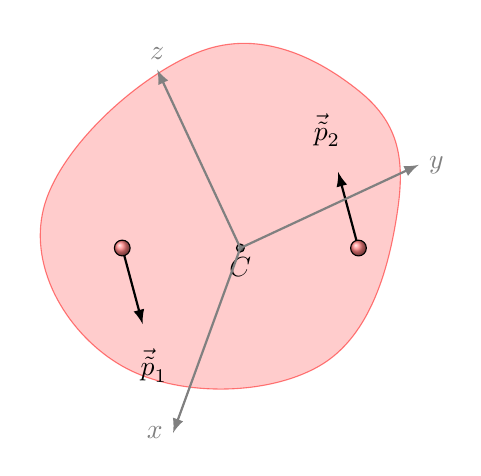
\begin{tikzpicture}
						\coordinate (O) at (0,0);
						\pgfmathsetmacro{\bodyang}{285}
						% ====== Bodyes ========
						\coordinate (B1) at (-1.5,0);
						\coordinate (B2) at (1.5,0);
						\coordinate (C) at (0,0);
						\pgfmathsetmacro{\ang}{20}
						% ====== System ========
						\pic at (C) {body};
						\draw[-latex, thick] (B1) -- +(\bodyang:1) node[anchor=\bodyang, pos=1.9] {$\vec{\tilde{p}}_1$};
						\draw[-latex, thick] (B2) -- +({\bodyang + 180}:1) node[anchor={\bodyang + 180}, pos=1.9] {$\vec{\tilde{p}}_2$};


						\foreach \i in {1,...,2} {\draw[ball color=red!50] (B\i) circle (0.1);}
						\draw[ball color=gray] (C) circle (0.05) node[below] {$C$};

						\begin{scope}[rotate = 25]
							\draw[thick, gray, -latex] (C) -- +(0,2.5) node[above, ] {$z$};
							\draw[thick, gray, -latex] (C) -- +(2.5,0) node[right] {$y$};
							\draw[thick, gray, -latex] (C) -- +(225:2.5) node[left] {$x$};
						\end{scope}
					\end{tikzpicture}
				\end{center}
			\end{column}
		\end{columns}
	}
\end{frame}


%=======================================================================================================

\title[Physics 1]{\huge\bfseries Motion of a Body with Variable Mass}
\begin{frame}
	\maketitle
\end{frame}

%=======================================================================================================
\begin{frame}{Rocket Propulsion}{}
	\begin{enumerate}
		\item There are many cases when the mass of a body varies in
		      the process of motion due to the continuous separation or
		      addition of matter (a rocket, a jet, a flatcar being loaded
		      in motion, etc.).
		\item The operation of a rocket depends upon the law of
		      conservation of linear momentum as applied to a
		      system of particles, where the system is the rocket plus
		      its ejected fuel.
	\end{enumerate}
	\begin{minipage}{0.5\linewidth}
		\begin{enumerate}
			\item 	The initial mass of the rocket plus all its fuel is $M + d m$ at time $t_i$
			      and speed $\vec v$
			\item The initial momentum of 	the system is $\vec p_i = (M + d m) \vec v$.
		\end{enumerate}
	\end{minipage}
	\begin{minipage}{0.4\linewidth}
		\includegraphics[width=\linewidth]{Rocket1}
	\end{minipage}
\end{frame}
%=======================================================================================================

%=======================================================================================================
\begin{frame}{Rocket Propulsion}{}
\begin{enumerate}
	\begin{minipage}{0.4\linewidth}
			\item At some time $t + d t$, the rocket’s mass has been reduced to $M$ and an amount of fuel, $d m$ has been ejected;
			\item The rocket’s speed has increased by $d \vec v$.
	\end{minipage}
	\begin{minipage}{0.5\linewidth}
		\includegraphics[width=\linewidth]{Rocket2}
	\end{minipage}
	\item Because the gases are given some momentum when they are ejected out of the engine, the rocket receives a compensating momentum in the opposite direction
	\item Therefore, the rocket is accelerated as a result of the <<push>> from the exhaust gases
	\item In free space, the centre of mass of the system (rocket plus expelled gases) moves uniformly, independent of 	the propulsion process.
\end{enumerate}
\end{frame}
%=======================================================================================================

%=======================================================================================================
\begin{frame}{Equation of motion of a body with a variable mass}{}
\only<1>{
	Change of momentum of system:
		\begin{multline*}
					d \vec p = \vec p_f - \vec p_i = \left[ M (\vec v + d\vec v) + dm_\mathrm{gas} \cdot \vec v_\mathrm{gas}\right]  - (M + dm_\mathrm{gas}) \vec v = \\
					 = \bcancel{M \vec v} + M d\vec v + dm_\mathrm{gas} \cdot \vec v_\mathrm{gas} -  \bcancel{M \vec v} - dm_\mathrm{gas} \cdot \vec v = \\
					= M d\vec v + dm_\mathrm{gas}(\vec v_\mathrm{gas} - \vec v) =  M d\vec v + dm_\mathrm{gas}\cdot \vec u,
		\end{multline*}
	{\small where $\vec u = \vec v_\mathrm{gas} - \vec v$ is the velocity of the added (separated) matter with 
	respect to the considered body, and $dm_\mathrm{rocket} = dm =  -dm_\mathrm{gas}$.}
}%
	According to the law of particle system motion, the momentum of a system may vary only due to \emph{external forces} $\frac{d \vec p}{dt} = \vec F^{ext}$, thus dividing this expression by $dt$, we obtain:
	\begin{equation*}
		\tcbhighmath[drop fuzzy shadow]{M \frac{d\vec v}{dt} = \vec F^{ext} + \frac{dm}{dt} \vec u}
	\end{equation*}
\only<1>{
	This is the fundamental equation of dynamics of a body with variable mass. It is referred to as the \textit{Meshchersky equation}. 
}
\only<2>{
The last term equation is referred to as the \emph{reactive force} or \emph{thrust}: 
\begin{equation*}
	\tcbhighmath[drop fuzzy shadow]{\vec R = \frac{dm}{dt} \vec u}.
\end{equation*}
This force appears as a result of the action that the added (separated) mass exerts on a given body. If mass is added, then $\frac{dm}{dt} > 0 $ and the vector $ \vec R $ coincides in direction with the vector $\vec u$; if mass is separated, $\frac{dm}{dt} < 0 $ and the vector $ \vec R $ is directed oppositely to the vector $\vec u$.
}
\end{frame}
%=======================================================================================================

%=======================================================================================================
\begin{frame}{The basic equation for rocket propulsion}{}
A rocket moves in the inertial reference frame in the absence of an external field of force $\vec F^{ext} = 0$, the gaseous jet escaping with the constant velocity $\vec u$ relative to the rocket. Lets find how the rocket velocity depends on its mass $m$ if at the moment of launching the mass is equal to $m_0$. 

In this case Equation of motion of a body with a variable mass yields $dv = u dm/m$. Integrating this expression with allowance made for the initial conditions, we get 
\begin{equation*}
	\tcbhighmath[drop fuzzy shadow]{v = - u \ln\frac{m_0}{m},}
\end{equation*}
this is the \emph{basic equation for rocket propulsion}, where the minus sign shows that the vector $\vec v$ (the rocket velocity) is directed oppositely to the vector $\vec u$. It is seen that in this case ($\vec u = \mathrm{const}$) the rocket velocity does not depend on the fuel combustion time: $\vec v$ is determined only by the ratio of the initial rocket mass $m_0$ to the remaining mass $m$.

\end{frame}
%=======================================================================================================

\end{document}